\qns{Bode Plots and Phasors}

\qcontributor{Tianrui Guo}

\begin{center}
\begin{circuitikz}
    \draw (0,1) node[ground] {}
      to[L=$L$,-*,i<=$I_L$] (2,1)
      to[R=$R_1$,i>=$I_R$] (5,1)
      to[short,-] (5,2.5);
    \draw (3.5,2.5) node[op amp, yscale=-1] (opamp) {}
      (opamp.+) to[R = $R_0$,-o] (0,3) node[left] {$V_{in}$};
    \draw (opamp.-) node[left] {}
      to[short,-] (2,2)
      to[short,-] (2,1);
    \draw (opamp.out) node[left] {}
      to[short,-*] (5,2.5) node[above] {$V_x$}
      to[R=$R_2$] (7,2.5)
      to[short,-o] (8,2.5) node[right] {$V_{out}$};
    \draw (7,2.5)
      to[C=$C$] (7,1) node[ground] {};
\end{circuitikz}

\end{center}
  
We found the transfer function of this circuit to be:
$$H(\omega) = \frac{R_1}{L} \frac{1 + j\omega \frac{L}{R_1}}{(j\omega)(1 + j\omega R_2 C)}$$
Using the following values:
$$R_0 = \SI{100}{\ohm}, R_1 = \SI{1}{\kilo\ohm}, L = \SI{1}{\micro\henry}, R_2 = \SI{100}{\kilo\ohm}, C = \SI{1}{\pico\farad}$$

\textbf{Plot its magnitude and phase Bode plots.}

\sol{
  
    \scalebox{0.9}{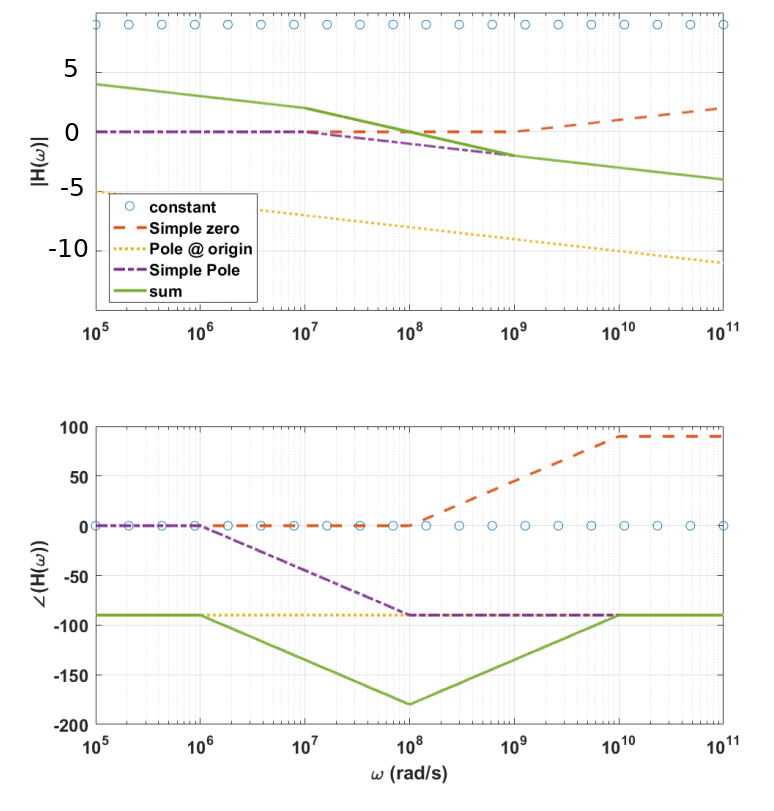
\includegraphics[scale=0.6]{figures/q_bode_a_fixed.png}}
    
}